\documentclass{standalone}
\usepackage{tikz}
\usetikzlibrary{arrows,positioning}
\begin{document}

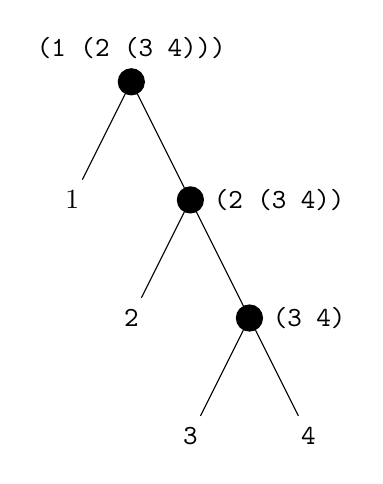
\begin{tikzpicture} [
	level 2/.style={sibling distance=15mm},
	internal/.style = {draw, circle, fill=black},
	leaf/.style = {minimum size = 5mm, fill=none},
]
\node [internal, label=\texttt{(1 (2 (3 4)))}] {}
	child {node [leaf] {1}}
	child {node [internal, label=right:\texttt{(2 (3 4))}] {}
		child {node [leaf] {\texttt{2}}}
		child {node [internal, label=right:\texttt{(3 4)}] {}
			child {node [leaf] {\texttt{3}}}
			child {node [leaf] {\texttt{4}}}}};
\end{tikzpicture}

\end{document}
